%1 - What is known

In the biosensor's community most findings and desicions in designed are achived 
through experimental analyses, trial and error procedures. Using
software to advice the design and manufacturing process can play a key role. In 
the world of plasmonics there are few softwares that are used to study Localized
Surface Plasmon Resonance. Among the most known softwares are COMSOL Multiphysics
a proprietary finite-element platform ({\color{red}cite COMSOL Multiphysics® v. 5.2. 
www.comsol.com. COMSOL AB, Stockholm, Sweden. NOT SURE HOW TO ADD THIS TO BIB} ), 
BEM++ ({\color{red}NOT SURE HOW TO CITE}) an open-source Boundary element method
library to solve time-harmonic Maxwell equations in 3D, and 
MNPBEM, an open-source Matlab toolbox for the simulation of metallic nanoparticles that
uses BEM and Hierarchical matrices \cite{Hohenester2018}. Besides, on the 
biosensing approach, the biomolecular electrostatic implementation of 
\pygbe \cite{CooperETal2016} allowed the study of ligand molecule orientation 
sensor \cite{CooperClementiBarba2015}.


%2 - What is UNknown, limitations and gaps


Most of these softwares solve full Maxwell equations which under certain
circumstances is no needed (long wave range limit), causing computational and 
memory expensive runs. Solving full maxwell equations when it is no necessary, 
limits also the problem-size that you can run as a user. Another caveat is the
 lack of open-source softwares that do not rely on licensed
languages. MNPBEM the open-source Matlab toolbox has recently evolved to a hierarchical
matrices and iterative solver approach reducing the computation time and memory
needs; however this software relies on a licensed language (Matlab) making its
accesibility restricted. Even though they are able to solve problems in teh order
of ten thousands, we can ensure that this amount of elements is good enough for 
the geometry sized. The lack of grid convergence analysis and error study in most of the 
softwares in the palsmonic community,
{\color{red}(I haven't find any of this in their papers, Chris what do you know about BEM++)}
force the user to believe in the obtained results without knowing their uncertainty. These
limitations prevent the development of a reproducible approach of any results obtained
with these softwares. 

%Limitation: 
%           - Software only study plasmonic assuming a non-lossy medium. 


%limitations - BEM++ {\color{red}Chris any input in this, limitations?}  
%              private are expensive and not accessible, 
%             matlab not free, 
%             no grid convergence analysis or error study, 
%             no reproducible framework 
%             problem size, geometry, and computation time


%Find structural details of analyte and nanoparticle, and the relative position between them.
%Studies that deal with real protein geometry.
%Gap: study this using fast, free-software dependencies and open source computer
%simulations. 


%3 - Burning question, experimental approach, why ours is new and diff (fill the gap)

Experiments suggest that the distance between the nanoparticle and the analyte 
affects the sensitivity of the sensor \cite{HaesETal2004}. However, this conclusions
are achived by a trial an error process, which leads to not enough understanding
on what is the relation between high dependance on sensitivity on distance in LSPR
biosensors. \pygbe most recent application \cite{ClementiETal2017} tends to 
bridge that gap providing via simulations, insights to guide the reasearch process.
The latest release of \pygbe extends the software to nanoplasmonics treating 
localized surface plasmon resonance (LSPR) quasi-statically \cite{MayergoyzZhang2007}.
Localized surface plasmon resonance (LSPR) biosensors measure the shift of 
plasmon resonace frequency in metallic nanoparticles when a target molecules 
binds to it. LSPR is an optical effect see Figure \ref{fig:lspr}, but electrostatics 
makes a good approximation in the long-wavelength limit. In this work we use
PyGBe's approach to study how the LSPR response changes in the presence of a 
biomolecule. To our knowledge, \pygbe is the only open-source software that uses a Tree code 
fast algorithm—O(N logN), for N unknowns, GMRES iterative solver; and hardware 
acceleration on GPUs to compute the extinction cross-sections of arbitrary 
geometries. The software \footnote{\url{https://github.com/barbagroup/pygbe}} is shared 
under the BSD 3-clause license and the development repository is available on 
Github.



\begin{figure}[h] %  figure placement: here, top, bottom, or page
   \centering
   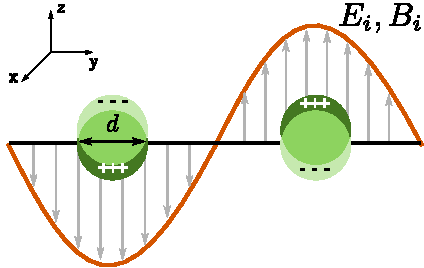
\includegraphics[width=0.35\textwidth]{lspr.pdf} 
   \caption{Localized Surface Plasmon Resonance (LSPR) scheme. LSPR is an 
            optical phenomenon that ocurrs when light shines on conductive 
            nanoparticles that are smaller than the wavelength of the incident 
            light. The free electrons on the surface of the nanoparticle are 
            excited by the incoming electric field oscillating with it and 
            creating plasmons}
   \label{fig:lspr}
\end{figure}




